\section{Verre doseur (4 points)}


En cuisine, il peut être pratique d'utiliser un verre doseur. Celui-ci permet de mesurer des masses de farine, de riz, de sucre et un volume de liquide.
Quelle quantité contient ce verre doseur, s'il s'agit :

\begin{center}
	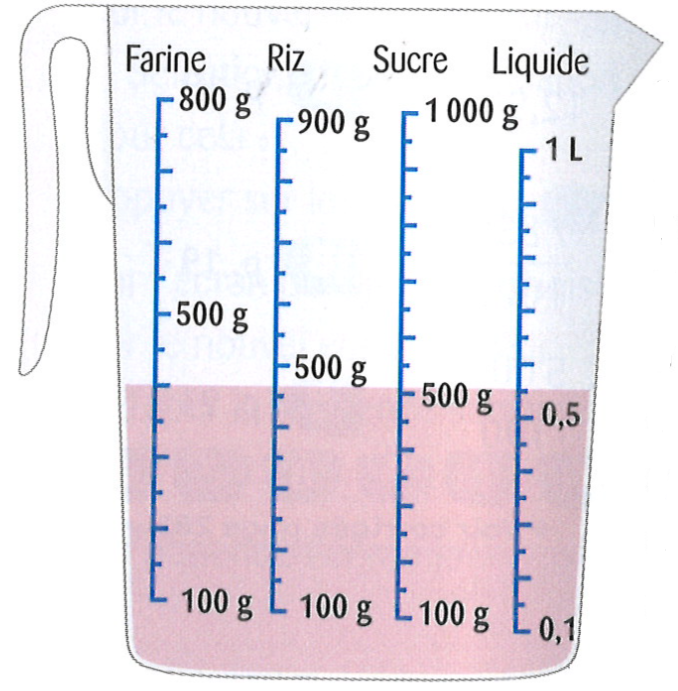
\includegraphics[scale=1]{img/verre}
\end{center}
\begin{questions}
	
	\begin{multicols}{2}
		
	\question[1] 
	
	de farine ? 
	\begin{solution}
		Le verre contient 400 grammes de farine.
	\end{solution}
	
	
	\question[1]
	
	de riz ?
	\begin{solution}
		Le verre contient 450 grammes de riz.
	\end{solution}
	
	\question[1]
	
	de sucre ? 
	\begin{solution}
		Le verre contient 500 grammes de sucre.
	\end{solution}
	
	\question[1]
	
	d'huile ?
	\begin{solution}
		Le verre contient \num{0.55} litres d'huile.
	\end{solution}
	\end{multicols}
	
\end{questions}